\documentclass{article}
\usepackage{sectsty}
\usepackage{url}
%\usepackage{enumitem}
\usepackage{enumerate}
\usepackage{xspace}
\usepackage{amssymb}
\usepackage{amsmath}
\usepackage{bussproofs}
\usepackage{graphicx}
\pagestyle{myheadings}
\markright{CS380C Compilers\\ Course Project Report}

\newcommand{\leakanalysis}[0]{LeakAnalysis.h\xspace}
\newcommand{\llvm}[0]{LLVM\xspace}
\newcommand{\crypt}[0]{glibc\_crypt\xspace}

\usepackage{titlesec}
\titleclass{\subsubparagraph}{straight}[\subparagraph]
\newcounter{subsubparagraph}
\renewcommand{\thesubsubparagraph}{\Alph{subsubparagraph}}
\titleformat{\subsubparagraph}[runin]{\normalfont\normalsize\bfseries}{\thesubsubparagraph}{1em}{}
\titlespacing*{\subsubparagraph} {\parindent}{3.25ex plus 1ex minus .2ex}{1em}


\title{\bf \Large An Implementation on Memory Leak Analysis by Contradiction}
\author{\normalsize Yige Hu (yh66596)}
%\date{\normalsize \today}
\date{}

\sectionfont{\fontsize{14}{17}\selectfont}

\begin{document}
\maketitle

\pagenumbering{arabic}

This report describes an implementation based on the algorithm proposed by
Orlovich and Rugina\cite{rugina} using \llvm. The paper discusses on both 
intra- and inter- procedural analysis. Due to the time constraint, only the
intra-procedural analysis is implemented in this work.

%\input{abstract}
\section{Introduction}
Memory leak is a standard cause of errors in low-level programming languages
such as C and C++. Those languages provide manual memory management and require
explicit deallocation of structures. The category of errors can eventually
causes a system to run our of memory, and is difficult to identify.

We describe a \llvm~\cite{llvm} implementation on an analysis which
can detect a set of errors caused by the memory leak. The implementation is
based on the algorithm proposed by Orlovich and Rugina~\cite{rugina}.

In this implementation we analysis and detect the potential memory leak error
by checking whether a statement can cause a potential loss of reference to a 
heap cell. The definition of a leaked (eroor) cell is given~\cite{rugina} as: the 
program or the run-time system doesn't reclaim its memory when the lifetime 
has ended.

The analysis works as a backward Dataflow analysis. For each statement that 
can cause a potential loss of heap cell reference, the analysis assume that 
it causes a loss of the last reference to the cell, and thus, an error cell
is formed. The analysis then release a detection probe to starts a backward 
Dataflow analysis from that programming point. If a contradiction is formed 
and the analysis reaches a bottom, the probe statement is proved to be safe. 
Otherwise, if the analysis reaches a $\top$, or it reaches the program entry, 
a warning of potential memory leak is released.

Section~\ref{s:algorithm} introduces the syntax, notations and algorithm
used by this implementation.

The evaluation~\ref{s:evaluation} is done through benchmarking. A set of 6 kinds
of microbenchmarks is used to show the correctness on different categories of
statements being analyzed. Then, two C programs from the GNU C Library source
code~\cite{glibc} are used to evaluate the performance on larger programs. No 
false positive are shown in the two GNU C programs.

%\input{motivation}
\section{Algorithm}
\label{s:algorithm}

We use the algorithm proposed by Orlovich and Rugina~\cite{rugina}. It is a 
backward Dataflow analysis, validating a statement's safety by searching for 
contradictions. It releases a detection probe for each suspicious statement 
that might lead to a loss of the last reference to a heap cell, assuming that 
a memory leak happens. A backward Dataflow analysis is immediately started from
that program point to check whether contradiction exist on all possible 
branches, which then proves that the probe statement is safe. If the Dataflow analysis 
reaches a $\top$ or the program entry is reached, the analysis reports a 
potential memory leak.


\subsection{Core Imperative Language}
\label{ss:semantics}

In this section we describe the core imperative language 
used by the algorithm, which helps better understand the later sections.

\paragraph{Syntax} 
\begin{align*}
  Statements s\in St s:: &= *e_0\gets e_1\ |\ *e\gets malloc\ |\ free(e)\ |\ \\
                         &     cond(e_0\equiv e_1)\ |\ return e\ |\ enter \\
  Expressions e\in E e:: &= n\ |\ a\ |\ *e\ |\ e.f\ |\ e_0 \oplus e_1 
\end{align*}

where, 
\begin{align*}
  n\in \mathbb{Z} &\text{  ranges over numeric constants $(NULL=0)$}, \\
  a\in \mathbb{A} &\text{  over symbolic addresses,} \\
  f\in \mathbb{F} &\text{  over structure fields,} \\
           \oplus &\text{  over arithmetic operators,} \\
           \equiv &\text{  over the comparison operators $=$ and $\ne$.}
\end{align*}


\paragraph{Mem(e) Function} 

The set $Mem(e)$ denotes the subexpressions of $e$ that represent memory 
locations. This set is defined recursively as follows:

\begin{align*}
  Mem(n) &= Mem(a)=\emptyset \\
Mem(e.f) &= Mem(e) \\
 Mem(*e) &={*e}\cup Mem(e) \\
Mem(e_0 \oplus e_1) &= Mem(e_0)\cup Mem(e_1)
\end{align*}

%The corresponding function in the implementation is the $getMem(e)$ 
%function in \leakanalysis.

Because of \llvm's SSA form, the expression context $\varepsilon$ described 
by the Rugina's paper~\cite{rugina} need not be considered.

\paragraph{Disjointness}

The analysis uses the points-to information from the Andersen's analysis 
to resolve alias and disjointness queries. 
An expression $e$ is disjoint from a region set 
$rs$, written $e\#rs$, if updates in any of the regions in $rs$ do not 
affect value of $e$:
\begin{align*}
e\#rs \iff \forall(*e')\in Mem(e). pt(e')\cap rs=\emptyset
\end{align*}

Where $pt(e')$ is the point-to set of the expression $e'$. 
A pointer analysis should be used to get such aliasing information. 
Flow-insensitive pointer analysis such as Andersen's~\cite{andersen} or 
Steensgaard's~\cite{steensgaard} can be used to get the two kinds of 
required information:

\begin{itemize}
  \item $Rgn$: the set of memory regions 
    (i.e. different regions model disjoint sets of memory locations);
  \item $pt(e)$: points-to information between regions.
\end{itemize}

In this work, we use Chen's implementation~\cite{chen} on the Andersen's 
analysis to get the above two information.
The regions are represented by the $AllocaInst$ or $CallInst$ to the $malloc()$ 
function in \llvm's SSA form. And the points-to set is represented by the 
set of the memory regions a pointer may point to.


\subsection{Backward Dataflow for Memory Leak}
\label{ss:dataflow}

This subsection describes the backward Dataflow in the memory leak analysis. 

\paragraph{Direction}

Backwards.

\paragraph{Flow Value and Error Cell Abstraction}

The flow value as well as the error cell is modeled by a triple of the form 
$(S,H,M)$, where:

\begin{itemize}
  \item $S\subseteq Rgn$ is the conservative set of regions that might hold 
    pointers to the error cell;
  \item $H$ is the Hit set, a set of expressions that point to the error cell; and 
  \item $M$ is the Miss set, a set of expressions that do not reference the cell.
\end{itemize}

$\bot$ means there is a contradiction, i.e. the statement is safe; 
$\top$ means there is a potential memory leak, and that the analysis should 
prompt a warning to the user.

\paragraph{Detection Probes and Initial Flow Values}

The analysis issues leak probes for the statements that can cause a potential 
memory leakage. Especially, at the following programming points:

\begin{enumerate}[(a)]
  \item Assignments: for each $*x_0\gets x_1$, build a dataflow triple 
    $(pt(e_0),\{*e_0\},\{e_1\})$;
  \item Allocations: each $*x_0\gets malloc$ is probed as $*x_0\gets 0$;
  \item Deallocations: for each $free(e)$, issue probes that correspond to a 
    sequence of assignments $*(e.f)\gets 0$, for each field $f$ of $e$. This 
    checks for leaks caused by freeing a cell that holds the last reference 
    to another cell.
\end{enumerate}

This implementation does not deal with the last case, since from the 
\llvm IR got by $clang$, the information of the fields in a structure is 
hidden and cannot be accessed directly.

\paragraph{Join Operation}

The partial ordering for the flow value is such that 
\begin{align*}
  (S_1,H_1,M_1)\sqsubseteq (S_2,H_2,M_2) & \text{  iif  } 
  S_1\subseteq S_2 \wedge H_1\supseteq H_2 \wedge M_1\supseteq M_2
\end{align*}

Therefore, the join operation is defined as:
\begin{align*}
  (S_1,H_1,M_1)\sqcup (S_2,H_2,M_2) &= (S_1\cup S_2,H_1\cap H_2,M_1\cap M_2)
\end{align*}


\paragraph{Transfer Function}

The transfer function differs on four categories of statements: assignment, 
allocation, deallocation and condition. A set of helper functions are used 
by the transfer functions:

\begin{align*}
  ImplicitMiss(e,(S,H,M)) &= (e=n) \vee (e=a) \vee (e=*n) \vee (e=n.f) \vee \\
                          &\ \ \ \ (e=*e' \wedge (S\cap pt(e')=\emptyset)) \\
  Miss(e,(S,H,M)) &= e\in M \vee ImplicitMiss(e,(S,H,M)) \\
Infeasible(S,H,M) &= \exists e \in H. Miss(e,(S,H,M)) \\
   Cleanup(S,H,M) &= (S,H,M'), \ where: \\
  M' &= {e|e\in M \wedge \urcorner ImplicitMiss(e,(S,H,M))} \\
\end{align*}

where $ImplicitMiss()$ detectes new misses;
$Miss()$ checks whether an expression is either in the Miss set or is a new miss; 
$Infeasible()$ indicates a contradiction;
$Cleanup()$ removes implicit miss to keep the dataflow facts as small as possible 
and avoid redundancy, while the correctness is reserved.

Four kinds of transfer functions are used corresponding to four kinds of 
statements under analysis:

\subsubparagraph{(1) Assignments}

\[
\Vert *e_0 \gets e_1 \Vert(S,H,M)=\begin{cases}
\bot& \text{if $Infeasible(S',H',M')$},\\
Cleanup(S',H',M')& \text{otherwise}.
\end{cases}
\]

%\begin{prooftree}
%  \AxiomC{$e\#\omega$}
%  \AxiomC{$e^{sgn}$}
%  \BinaryInfC{$^{sgn}e$}
%\end{prooftree}

\begin{figure}
  \centering
  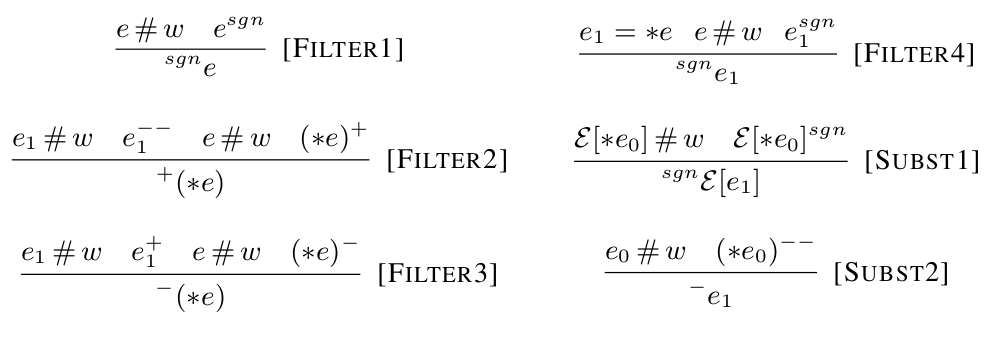
\includegraphics[width=1.0\columnwidth]{figs/rules_assignment}
   \caption{Deduction rules for the analysis on assignments.}
   \label{fig:rule_ass}
\end{figure}

where $S'=S\cup pt(e_0)$, and $H',M'$ are derived using the deduction rules 
described in Figure~\ref{fig:rule_ass}, where $e^+$ and $e^-$ represent 
respectively $e\in H$ and $e\in M$ (hit/miss expressions in the post-state); 
$^+e$ and $^-e$ for $e\in H'$ and $e\in M'$ (hit/miss expressions in the 
pre-state); and $e^{--}$ denotes that $Miss(e,(S,H,M))$. The set $\omega$ is 
the set of regions potentially written by the assignment: $w=pt(e_0)$. Hence,
an expression has the same value before and after the statement if it is 
disjoint from $\omega$. 
[FILTER 1-4] judge which expressions are reserved from the post-state to the 
pre-state. [SUBST 1-2] generate new elements in the Hit and Miss sets.


\subsubparagraph{(2) Allocations}

\[
\Vert *e_0 \gets malloc \Vert(d)=\begin{cases}
\bot& \text{if $UnaliasedHit \wedge (*e_0 \in H \wedge e_0\#\omega)$},\\
\Vert *e_0 \gets 0 \Vert (d)& 
  \text{if $UnaliasedHit \vee (Miss(*e_0,d) \wedge e_0\#\omega)$},\\
\top& \text{otherwise}.
\end{cases}
\]

where $d=(S,H,M)$, $\omega=pt(e_0)$, and 
$UnaliasedHit=\exists(*e)\in H:pt(e)\cap\omega =\emptyset$.
It denotes that there is some expression unaliased to $*e_0$ also 
references the cell. Thus, if it holds as well as $(*e_0)^+$, a contradiction
occurs. Or, if there is evidence that the error cell has not been 
allocated at this site, it proceeds past this statement, treating the 
allocation as a nullification $*e_0 \gets 0$.

\subsubparagraph{(3) Deallocations}

\[
\Vert free(*e_0) \Vert(S,H,M)=\begin{cases}
\bot& \text{if $e \in H$},\\
(S,H,M)& \text{if $(Miss(e,(S,H,M))$},\\
(S,H,M\cup {e})& \text{otherwise}.
\end{cases}
\]

A contradiction occurs if the reference lost is a reference to a cell that has 
already been freed, which is actually not an error. Otherwise, the analysis 
knows that $e$ misses in the pre-state.

\subsubparagraph{(4) Conditions}

\[
\Vert cond(e_0\equiv e_1)\Vert(S,H,M)=\begin{cases}
\bot& \text{if $Infeasible(S,H",M")$},\\
Cleanup(S,H",M")& \text{otherwise}.
\end{cases}
\]

\begin{figure}
  \centering
  
\includegraphics[width=1.0\columnwidth]{figs/rules_cond}
   \caption{Deduction rules for the analysis on conditions.}
   \label{fig:rule_cond}
\end{figure}

where $H"=H\cup H'$, $M"=M\cup M'$, $H'$ and $M'$ are the new hit and miss 
expressions derived using the deduction rules in Figure~\ref{fig:rule_cond}. 
The conditions can help derive new hit and miss expressions in the pre-state 
because they infer that the (in)equality is succeeded in the post-state.

\section{Implementation Details and Improvements}
\label{s:implementation}

The analysis uses a worklist-based Dataflow algorithm. 
This section describes some implementation details. Also, some other constraints 
are added to decrease the false positives.

\paragraph{The Representation of Pointers in the Hit Set}

One difference between the implementation and the paper's description is that 
instead of storing the pointer ${*e_0}$,
we allow the Hit set in the dataflow value to store either ${*e_0}$ or its 
address ${e_0}$ to represent the pointer. This is to adapt \llvm's SSA form 
representation of the store instructions, from which only the address of the 
pointer can be get, instead of a concrete representation of a pointer itself. 
e.g. When an variable address is stored into a pointer, the SSA form 
representation will be:
\begin{align*}
store i32* \%1, i32** \%a, align 8
\end{align*}
where $\%a$ is the address of the pointer $a$.

Accordingly, changes are made into the transfer functions and the deduction 
rules to consider both the cases when either a pointer's value or a pointer's 
address is stored to represent the pointer's existence in the Hit set. 
Such changes also guarantee that the new rules are equivalent to the rules in 
the Rugina~\cite{rugina} paper. Take the deduction rule $[SUBST2]$ in 
Figure~\ref{fig:rule_ass} 
as an example, its new representation in our implementation will 
be two separate rules:
\begin{prooftree}
  \AxiomC{$e_0\#\omega$}
  \AxiomC{$\exists(*e')\in M$}
  \AxiomC{$e'=e_0$}
  \TrinaryInfC{$^-e_1$}
\end{prooftree}
and
\begin{prooftree}
  \AxiomC{$e_0\#\omega$}
  \AxiomC{$S\cap pt(e_0)=\emptyset$}
  \BinaryInfC{$^-e_1$}
\end{prooftree}


\paragraph{Branches, Worklist and Exit Conditions}

When there are branches in the program, the analysis reaches a $\bot$ only if 
contradiction exist in all branches. The Rugina~\cite{rugina} paper does not 
describe how to handle this in details. So in this paragraph we will have a 
short discussion on the details of worklist, branches and exiting conditions.

Firstly, we added another boolean value $Contr$ into the flow value to 
represent a contradiction has been discovered. And the join operation is 
extended like this:
\begin{align*}
  (S_1,H_1,M_1,Contr_1) &\sqcup (S_2,H_2,M_2,Contr_2) \\
  = (S_1\cup S_2,H_1\cap H_2, & M_1\cap M_2,Contr_1\wedge Contr_2)
\end{align*}

When a probe statement is reached, the analysis start a backward Dataflow 
analysis by inserting the basic block where 
the probe resides in. Then, the analysis continues to work until one of the 
following conditions is met:
\begin{itemize}
  \item A $\top$ is reached: the analysis exit and prompt an warning of 
    potential memory leak;
  \item A $\bot$ is reached in the local basic block of the probe: 
    the probe is proved to be safe and the analysis exits without checking all 
    the branches;
  \item A $\bot$ is reached in the entry block from all of its successors:
    the probe is proved to be safe and the analysis exits;
  \item The entry point is reached and the worklist is empty.
\end{itemize}

If a basic block gets a $\bot$ through the meet operation on all its successors,
or if a new $\bot$ is reached inside a basic block, we will skip the analysis on 
the remaining statements in that block, and add its predecessors into the 
worklist.

Also, to avoid redundent loops for the convergence of the dataflow values, 
we only insert a predecessor $BB_p$ of a basic block $BB_s$ iff. they meets 
all the following conditions:
\begin{itemize}
  \item $BB_s$ has been changed;
  \item The $Contr$ in $BB_p$'s out value has not been set to $true$ before.
\end{itemize}


\paragraph{Improvements}

Besides the cases discussed in the Rugina~\cite{rugina} paper, we also exclude 
some other cases which can generate false positives;

\begin{itemize}
  \item The first assignment of an uninitialized pointer;
  \item The storage into a non-pointer type;
\end{itemize}

\section{Evaluation}
\label{s:evaluation}

%\input{related}
\section{Conclusions}

We have implemented a memory leak detector based on an iterative Dataflow 
algorithm using 
a work-list, which is proposed by Orlovich and Rugina~\cite{rugina}. The analysis 
starts a backward Dataflow for each probe statements to disprove its negation. 
A set of six categories of microbenchmarks are tested to show the correctness 
of the implementation. We have also examined two GNU C library programs with no 
false positive. Due to the time constraint, the implementation only completes 
the intra-procedural analysis. Also, not enough middle- or large-scale C 
programs have been tested as benchmarks.

%\input{acknowledgements}
% Conference macros
% include this in enclosing document for long conference names
\def\longconferencenames{}

%  Use this one for the cv notes
%\def\includecvnotes{}
%\def\includebionotes{}

\newcommand{\osaconfname}[3]{
\ifx\longconferencenames\undefined
\newcommand{#1}[0]{{#2}}
\else
\newcommand{#1}[0]{{#3}}
\fi
}

\newcommand{\cvnote}[1]{
\ifx\includecvnotes\undefined
%
\else
{#1}%
\fi
}


\newcommand{\bionote}[1]{
\ifx\includebionotes\undefined
%
\else
{#1}%
\fi
}


\osaconfname{\sas}{SAS'06}{Proceedings of the 13th International Conference
on Static Analysis (SAS'06)}

\osaconfname{\podc}{PODC}{Proceedings of the ACM symposium on Principles of
distributed computing (PODC)}

\osaconfname{\asplos}{ASPLOS}{{Proceedings of the ACM International Conference on Architectural Support for Programming Languages and Operating Systems (ASPLOS)}}

\osaconfname{\spaa}{SPAA}{{Proceedings of the ACM symposium on Parallelism in algorithms and architectures (SPAA)}}

\osaconfname{\osdi}{OSDI}{{Proceedings of the USENIX Symposium on Operating Systems Design and Implementation (OSDI)}}

\osaconfname{\disc}{DISC}{{Proceedings of the International Conference on Distributed Computing (DISC)}}

\osaconfname{\usenixatc}{USENIX}{{Proceedings of the USENIX Annual Technical Conference}}
\osaconfname{\usenixsec}{USENIX Security}{{Proceedings of the USENIX Security Symposium}}

\osaconfname{\pldi}{PLDI}{{Proceedings of the ACM SIGPLAN conference on Programming language design and implementation (PLDI)}}

\osaconfname{\computer}{Computer}{{IEEE Computer}}

\osaconfname{\sosp}{SOSP}{{Proceedings of the ACM SIGOPS Symposium on Operating Systems Principles (SOSP)}}

\osaconfname{\isca}{ISCA}{{Proceedings of the ACM IEEE International Symposium on Computer Architecture (ISCA)}}

\osaconfname{\csaw}{CSAW}{{Proceedings of the ACM Workshop on Computer Security Architecture (CSAW)}}

\osaconfname{\wddd}{WDDD}{{Proceedings of the Workshop on Duplicating, Deconstructing, and Debunking (WDDD)}}

\osaconfname{\vldb}{VLDB}{{Proceedings of the International Conference on Very Large Databases (VLDB)}}

\osaconfname{\toplas}{TOPLAS}{{ACM Transactions on Programming Languages and Systems (TOPLAS)}}

\osaconfname{\tocs}{TOCS}{{ACM Transactions on Computer Systems (TOCS)}}

\osaconfname{\ppopp}{{PPoPP}}{{Proceedings of the ACM SIGPLAN Symposium on Principles and Practice of Parallel Programming (PPoPP)}}

\osaconfname{\jpdc}{J. Parallel Distrib. Comput.}{{Journal of Parallel and Distributed Computing}}

\osaconfname{\ismm}{ISMM}{{Proceedings of the ACM International Symposium on Memory Management (ISMM)}}

\osaconfname{\cacm}{CACM}{{Communications of the ACM (CACM)}}

\osaconfname{\hpca}{HPCA}{{Proceedings of the IEEE International Symposium on High-Performance Computer Architecture (HPCA)}}

\osaconfname{\transact}{TRANSACT}{{Proceedings of the ACM SIGPLAN Workshop on Transactional Computing (TRANSACT)}}

\osaconfname{\iiswc}{IISWC}{{Proceedings of the IEEE International Symposium on Workload Characterization (IISWC)}}

\osaconfname{\tpds}{IEEE Trans, Parallel Distrib. Syst.}{{IEEE Transactions on Parallel and Distributed Systems}}

\osaconfname{\osr}{OSR}{{ACM Operating Systems Review}}

\osaconfname{\nsdi}{NSDI}{{Proceedings of the USENIX Symposium on Networked Systems Design and Implementation (NSDI)}}

\osaconfname{\cc}{CC}{{Proceedings of the International Conference on Compiler Construction (CC)}}

\osaconfname{\surveys}{ACM Comput. Surv.}{{ACM Computing Surveys}}
\osaconfname{\icde}{IDCE}{{Proceedings of the IEEE International Conference on Data Engineering (ICDE)}}
\osaconfname{\fast}{FAST}{{Proceedings of the USENIX Conference on File and Storage Technologies (FAST)}}
\osaconfname{\eurosys}{{E}uro{S}ys}{{Proceedings of the ACM European Conference on Computer Systems ({E}uro{S}ys)}}
\osaconfname{\hotos}{HotOS}{{Proceedings of the USENIX Workshop on Hot Topics in Operating Systems (HotOS)}}
\osaconfname{\oopsla}{OOPSLA}{{Proceedings of the ACM SIGPLAN Conference on Object-Oriented Programming, Systems, Languages, and Applications (OOPSLA)}}
\osaconfname{\ndss}{NDSS}{{Proceedings of the Network and Distributed System Security Symposium (NDSS)}}
\osaconfname{\oakland}{Oakland}{{Proceedings of the IEEE Symposium on Security and Privacy (Oakland)}}
\osaconfname{\ispass}{ISPASS}{{Proceedings of the IEEE International Symposium on Performance Analysis of Systems and Software (ISPASS)}}

\osaconfname{\europar}{{E}uro{P}ar}{{Proceedings of the European Conference on Parallel Programming ({E}uro{P}ar)}}

\osaconfname{\sigcse}{{SIGCSE}}{{Proceedings of the ACM SIGCSE technical symposium on Computer science education (SIGCSE)}}

\osaconfname{\ccs}{{CCS}}{{Proceedings of the ACM Conference on Computer and Communications Security (CCS)}}

\osaconfname{\veeconf}{{VEE}}{{Proceedings of the International Conference on Virtual Execution Environments (VEE)}}

\osaconfname{\lisa}{{LISA}}{{Proceedings of the Large Installation System Administration Conference (LISA)}}

\osaconfname{\sac}{{SAC}}{{Proceedings of the ACM Symposium on Applied computing (SAC)}}

\osaconfname{\acsac}{{ACSAC}}{{Proceedings of the Annual Computer Security Applications Conference (ACSAC)}}

\osaconfname{\sacmat}{SACMAT}{{Proceedings of the ACM Symposium on Access Control Models and Technologies (SACMAT)}}
\osaconfname{\hotsec}{HotSec}{{Proceedings of the USENIX Workshop on
    Hot Topics in Security (HotSec)}}
\osaconfname{\hotnets}{HotNets}{{Proceedings of the ACM Workshop on Hot
    Topics in Networks (HotNets)}}
\osaconfname{\stc}{STC}{{Proceedings of the ACM workshop on Scalable Trusted Computing (STC)}}
\osaconfname{\tissec}{TISSEC}{{ACM Transactions of Information and System Security (TISSEC)}}
\osaconfname{\gpc}{GPC}{{Proceedings of the International Conference on Grid and Pervasive Computing (GPC)}}

\osaconfname{\microkernels}{Microkernels}{{Proceedings of the USENIX Workshop on Microkernels and Other Kernel Architectures}}
\osaconfname{\ares}{{ARES}}{{Proceedings of the International Conference on Availability, Reliability and Security (ARES)}}
\osaconfname{\winter}{{USENIX Winter}}{{Proceedings of the Winter USENIX Conference}}
\osaconfname{\otm}{{OTM}}{{On the Move to Meaningful Internet Systems (OTM)}}
\osaconfname{\jacm}{{JACM}}{{Journal of the ACM}}
\osaconfname{\icdcs}{{ICDCS}}{{Proceedings of the International
    Conference on Distributed Computing Systems}}

\osaconfname{\sigcomm}{{SIGCOMM}}{{Proceedings of the ACM SIGCOMM
    Conference on Applications, Technologies, Architectures, and
    Protocols for Computer Communications}}

\osaconfname{\socc}{{SoCC}}{{Proceedings of the ACM Symposium on Cloud Computing}}


\footnotesize
\bibliographystyle{abbrv}
\bibliography{bibliography}

\end{document}
